
For stocks with analytical assessments (category 1 and 2 stocks), MSY reference points are used by the advice rules applied by ICES to give advice consistent with the objective of achieving MSY. For stocks in categories 3 and 4 ICES uses MSY proxy reference points are used as part of a Precautionary Approach to provide advice on the status of the stock and exploitation. The $F_{MSY}$ proxy corresponds to the exploitation rate that will provide maximum long-term yield. The $MSY_{Btrigger}$ proxy corresponds to the stock size that triggers a cautious response; i.e. advice on a reduced fishing mortality relative to the $F_{MSY}$ proxy to allow the stock to rebuild. 

A number of potential length based reference point comparisons have been identified by ICES (see Figure |%\label{fig:lib}) for stocks in categories 3 and 4\footnote{http://ices.dk/sites/pub/Publication Reports/Guidelines and Policies/16.04.03.02_Category_3-4_Reference_Points.pdf}


%\newpage
%\begin{figure}[h]\centering
%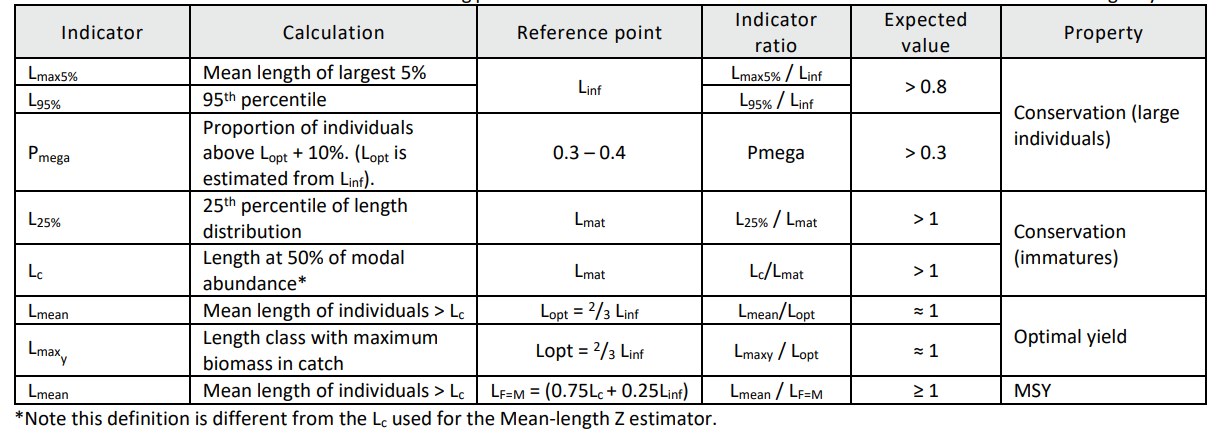
\includegraphics[width=\textwidth]{figs/lib.png}
%\caption{Length based indicators.}
|%\label{fig:lib}
|%\end{figure}

For stocks with $MSY$ proxy reference points not derived from an assessment model, ICES uses a generic rule of the form 
 
\begin{equation}
C_{y+1}=C_{current}rfb
 \end{equation}

where $C_{current}$ is the catch either in the most recent year available (typically $y-1$) or the average over a number of recent years (e.g. 
$y-n, ... ,y-1$), $r$ should account for the trend in stock biomass ($r>0$; with $r=1$ if there is no trend), $f$  is a proxy for the ratio $F_{MSY}/$(current explotation) and $b=$ min(1,proxy for the ratio (current stock size)/($MSY_{Btrigger}$)). The later is in effect a hockey stick type HCR. 


The advisory rule (AR) most commonly used by ICES for category 3 stocks, is the so-called \textit{2 over 3} rule of this type is $C_{current}=$ most recent advice provided for the stock, $r=$ (average of stock size indicator in the last 2 years)/(average of stock size indicator in the 3 preceding years), $f=1$ and $b=1$. The \textit{2 over 3} ICES rule also incorporates  a  limit  on  maximum  interannual  change  (20\%  uncertainty  cap,  to  protect  against  changes  in  advice  not  related  to  underlying  population  dynamics )  and  a  PA buffer (20\% additional reduction, which is applied if stock status relative to reference 
points is bad or unknown, with some exceptions); the PA buffer is not applied every year, but at certain time intervals.

Usage of the value 1 for the factors $f$ and $b$ and  in the ICES \textit{2 over 3} rule just described is related  to  the  fact  that  no  MSY  proxy  reference  points  have  been  available  for  ICES  
category  3  and  4  stocks  until  recently  and,  there fore,  it  was  not  possible  to  calculate values for $f$ and $b$  taking into account reference points. Within the framework of the generic catch rule in (3.2.1.1), WKMSYCat34 proposes the following “first candidates” for an ICES MSY advice rule, making use of the now available MSY proxy reference points.

  
Usage of the value 1 for the factors $f$ and $b$ in the ICES \textit{2 over 3} rule just described is values for $f$ and $b$ taking into account reference points.

\textbf{Options for $r$:}

a )  \textit{2 over 3}, i.e. $r$ = (average of stock size index in the 2 most recent years)/(average of stock indexin the predeeding three years). Note that this waay of setting $r$ essentially corresponds to a 2.5 year interval for the index change; this might be suitable for biennial or triennial advice, but may possibly be overly responsive for annual advice.
b ) $r$ = exp{ w * (slope of a straight line fitted to the logarithm of the stock size index in the last 5 years) }. Values 1 or 2, essentially corresponding to an interval of 1 or 2 years for the index to be explored.
c )  More sophisticated options could be considered for $r$ (e.g. optimise one-step, e.g. one step ahead prediction, for example by using a biomass dynamic model to smooth a) or b).

The options above are for category 3 stocks. For category 4 stocks, use $r$ = 1. 



\textbf{Options for $f$:} 

a ) $f = L_{current}/L_{F=M}$, where L denotes the mean length of catch above the length of first capture ($L_c$), and $L_{F=M}$ is calculated using the Beverton-Holt equilibrium formula provided below.
b ) $f = M/(Z_{current}-M)$, 
where $Z_{current}$ is calculated from $L_{current}$ using the Beverton-Holt equilibrium formula provided below.
c ) $f = F_{0.1}/(Z_{current}-M)$, where $Z_{current}$ is calculated from the Gedamke \& Hoenig (2006) method, potentially with information on effort, and $F_{0.1}$ from length-based Yield-Per-Recruit analysis with 

comparable assumptions to the calculation in the denominator.  
d )  More sophisticated options for $f$ (e.g. based on the LB-SPR method (Hordyk et al., 2015a, b, c), or S6 (Kokkalis et al., 2017)). 

In the options that use $L_{current}$ or $Z_{current}$, \textit{current} refers to the most recent year available or the average (of L or Z) over a number of recent years. The number of recent years used to specify \textit{current} is to be investigated The Beverton-Holt equilibrium formula for mean length of the catch above the length 

of first capture ($L_c$) is as follows: 

$L_{F} = \frac{L\infty +\frac{F+M}{K}L_c}{1+\frac{F+M}{K}} =
         \frac{L\infty +\frac{Z}{K}L_c}{1+\frac{Z}{K}} \Rightarrow L_{F=M} = \frac{L\infty +\frac{2M}{K}L_c}{1+\frac{2M}{K}}$

The options above are applicable to stocks in categories 3 or 4. 

Generic MSE testing (as described in Section 4 of this report) in principle compares all possible options for $f$, whereas stock-specific testing would select a particular option depending on the method that has  been used to calculate the MSY proxy reference point for the stock: 


In  cases  where  the  mean  length  of  the  catch  (above  $L_c$)  calculated  from the Beverton-Holt equilibrium formula is used to derive the FMSY proxy, and this proxy corresponds to F=M, then use options a or b.  In  cases  where  the  Gedamke  \&  Hoenig  method  (with  potential  information about effort) is used to derive the FMSY proxy, and this proxy corresponds to F=F0.1, then use option c. 

\textbf{Options for b:} 

Most of the methods used by ICES to set proxy MSY reference points for stocks in categories 3 and 4, provide proxies for FMSY but not for MSY Btrigger. Therefore, unlike for 

$f$, there are generally no MSY Btrigger proxies than can readily be used for $b$ in the generic catch rule. Two options are suggested for $b$ by WKMSYCat34 

a ) $b= min\lbrace{ 1,\frac{l_{current}}{l_{trigger}}\rbrace}$

with $L_{trigger}$ = w $I_{lim}$ (where w≥1). The value of w and If one could identify an $I_{lim}$ value (i.e. a limit value for the stock size index; it is 

not expected that we will have formally set Blim for stocks in category 3), either from stock and recruitment indices (e.g. based on survey data) or, in the absence of 

the number of recent years used to specify \textit{current} are to be investigated. 

 
b )  b = 0.8 (PA buffer: 20\%, applied every e.g. 4 years) 

that, as the minimum of the observed index series, the suggestion is to set $L_{trigger}$ = 1.4 $I_{lim}$. 

\textbf{Options for $𝑪_{current}$:}

Stocks in category 3 should use option a, and stocks in category 4 should use option b. 

a )  WKMSYCat34 discussed whether it was more appropriate to use “current catch“ or “current advice“ in the rule (advice and catch would ideally be identical, but this is rarely the case in reality). It was concluded that catch, rather than advice, was the most appropriate option to use in the rule given the definition of the factor $f$ included in the rule (see 3.2.1.1). The purpose of the factor $f$ is to modify exploitation from the current level to the level 

corresponding to the FMSY proxy, and exploitation relates to catch rather than to advice, when the two differ. 

b )  More sophisticated options could be considered (e.g. methods that compare actual catches with advice, or that are able to deal with the fact that the factor $f$ will  generally  be  slow-reacting,  which  can  negatively  affect  the  performance of the rule) 

As already noted, the most appropriate choice for the number of recent years used to specify “current“ is to be investigated, and this could be done via MSE. In principle, it is expected that, for a given stock, \textit{current} would be defined in the same way for Ccurrent and for the factor f , as both directly relate to exploitation. The factor b relates to a stock size indicator and a different definition of “current“ might be more appropriate in that case.  


\href{http://ices.dk/sites/pub/Publication Reports/Expert Group Report/Fisheries Resources Steering Group/2019/WKLIFEIX/WKLIFE_IX_2019.pdf#page=30}{wklifeix: 4 Length-based approaches}

\href{http://ices.dk/sites/pub/Publication Reports/Expert Group Report/Fisheries Resources Steering Group/2019/WKLIFEIX/WKLIFE_IX_2019.pdf#page=58}{[wklifeix: ROC]}

\href{http://ices.dk/sites/pub/Publication Reports/Expert Group Report/Fisheries Resources Steering Group/2019/WKLIFEIX/WKLIFE_IX_2019.pdf#page=100}{[wklifeix: hake]}

The International Council of the Exploration of the Sea (ICES)** is in the process of developing methods to identify MSY proxy reference points for data-limited stocks ([WKLIFE](http://ices.dk/sites/pub/Publication Reports/Expert Group Report/Fisheries Resources Steering Group/2019/WKLIFEIX/WKLIFE_IX_2019.pdf)). The service provider is required to contribute to this process by proposing and testing new assessment models and methods of establishing reference points and will be expected to attend up to 4 one-week meetings at ICES headquarters in Copenhagen. However there are key differences with the ICES approach. Since this research contract will include stocks not currently assessed by ICES; focusing on the available data for each stock first and on the methods second; the ICES approach focuses on the methods first and then applies a limited number of methods to a large number of stocks.


